\documentclass[conference]{IEEEtran}
\IEEEoverridecommandlockouts

\usepackage{cite}
\usepackage{amsmath,amssymb}
\usepackage{graphicx}
\usepackage{booktabs}
\usepackage{xcolor}
\usepackage{tikz}
\usetikzlibrary{arrows.meta,positioning,fit}
\usepackage[hidelinks]{hyperref}

\begin{document}

\title{Do Clinic Arm Assessments Reflect Arm Use at Home After Stroke?\\
A Wearable-Sensor Study of Ecological Validity}

\author{\IEEEauthorblockN{Bijyeta Maharjan}
\IEEEauthorblockA{Mount Holyoke College\\
\texttt{bmaharjan@umass.edu}}}

\maketitle

\begin{abstract}
Upper-limb recovery after stroke is usually judged from structured, in-clinic
assessments, yet the outcome that matters to patients is how much they use their
arms in daily life. We test whether sensor-derived measures of arm activity
recorded in the lab reflect activity recorded at home. Eighteen chronic stroke
survivors wore bilateral wrist accelerometers during a structured lab session and
over multiple days of free-living home recording. From both contexts we computed
seven measures of arm-use intensity, duration, and between-arm asymmetry. Because
home recordings contain long rest and non-wear periods that lab sessions do not,
we swept an activity threshold to remove inactive epochs, selecting the threshold
at which lab and home intensities were statistically comparable while
between-participant agreement remained strongest. Lab–home agreement was then
assessed with Pearson correlation, $R^2$, and paired $t$-tests, and sensor
measures were related to standard clinical scores (FMA, MAL, WMFT) with Spearman
correlation. Lab measures predicted home use of the stroke-affected arm but not of
the unaffected arm, indicating that in-clinic sensor assessment is a reasonable
proxy for real-world use of the impaired limb only.
\end{abstract}

\begin{IEEEkeywords}
stroke rehabilitation, wearable sensors, accelerometry, upper limb,
ecological validity, real-world arm use
\end{IEEEkeywords}

% ────────────────────────────────────────────────────────────────────────────
\section{Introduction}

Clinicians track upper-limb recovery after stroke with standardized assessments
performed in the clinic, such as the Fugl-Meyer Assessment (FMA)~\cite{fuglmeyer1975}
and the Wolf Motor Function Test (WMFT)~\cite{wolf2001}, sometimes complemented by
self-report of daily use through the Motor Activity Log (MAL)~\cite{uswatte2006mal}.
These tools measure what a person \emph{can} do under controlled conditions. They do
not directly measure what the person \emph{does} at home, and prior work shows that
gains in clinical capacity do not always translate into more arm use in daily
life~\cite{rand2012,waddell2017}.

Wrist-worn accelerometers make it possible to measure arm activity continuously,
both in the clinic and during everyday life~\cite{uswatte2006accel,bailey2014}.
This raises a practical question: if a clinician records sensor data during a
short, structured lab session, does it tell them anything about how the patient
uses each arm at home?

This project addresses that question directly. The contributions are:
\begin{itemize}
  \item A study design pairing in-lab and multi-day home recordings from the same
        participants, with identical sensor processing in both contexts.
  \item An empirical activity-threshold optimization that makes lab and home
        intensities comparable despite rest and non-wear time at home.
  \item A limb-specific analysis of lab–home agreement and of the relationship
        between sensor measures and clinical scores.
\end{itemize}

% ────────────────────────────────────────────────────────────────────────────
\section{Methods}

\subsection{Participants and Recordings}

Eighteen chronic stroke survivors were included in the final analysis.
Participants were excluded if a wrist sensor recording was missing, if the home
recording was empty, or if the in-lab session was unavailable. Each participant
wore accelerometers on both wrists (and fingers) during (i) a structured in-lab
session of upper-limb tasks and (ii) several days of free-living recording at home.
Sensors were labelled as \emph{affected} or \emph{less affected} using each
participant's clinically documented affected side. This analysis uses the wrist
sensors.

\subsection{Signal Processing}

The same pipeline was applied to lab and home data (Fig.~\ref{fig:pipeline}).
Each sensor stream was interpolated onto a uniform 50\,Hz time base and aligned
across sensors. Acceleration magnitude was band-pass filtered (6th-order
zero-phase Butterworth, 0.25--10\,Hz) to remove gravity, drift, and high-frequency
noise, then rectified and averaged over non-overlapping 1\,s epochs (50 samples).
Multi-day home segments were concatenated into a single epoch series per
participant.

\begin{figure}[t]
\centering
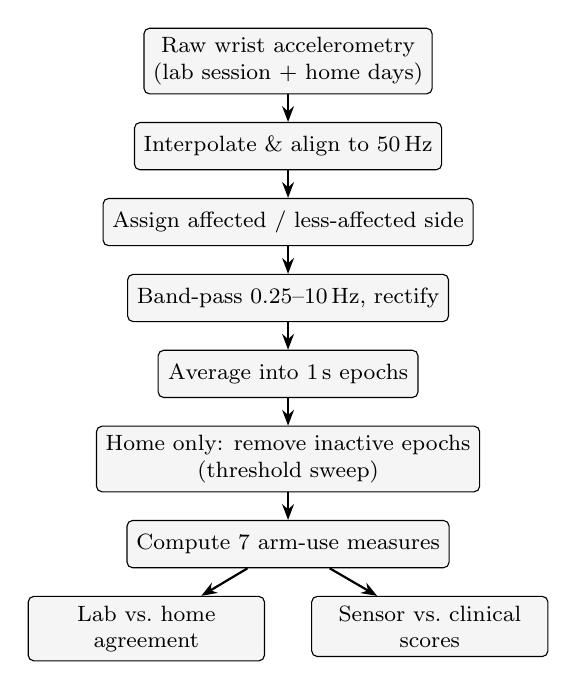
\begin{tikzpicture}[
  node distance=3.5mm,
  box/.style={draw, rounded corners=2pt, align=center, font=\footnotesize,
              minimum width=33mm, minimum height=6mm, fill=gray!8},
  arr/.style={-{Stealth[length=2mm]}, thick}]
  \node[box] (raw) {Raw wrist accelerometry\\(lab session + home days)};
  \node[box, below=of raw] (interp) {Interpolate \& align to 50\,Hz};
  \node[box, below=of interp] (assign) {Assign affected / less-affected side};
  \node[box, below=of assign] (bpf) {Band-pass 0.25--10\,Hz, rectify};
  \node[box, below=of bpf] (epoch) {Average into 1\,s epochs};
  \node[box, below=of epoch] (thr) {Home only: remove inactive epochs\\(threshold sweep)};
  \node[box, below=of thr] (meas) {Compute 7 arm-use measures};
  \node[box, below=of meas, xshift=-18mm, minimum width=30mm] (labrw) {Lab vs.\ home\\agreement};
  \node[box, below=of meas, xshift=18mm, minimum width=30mm] (clin) {Sensor vs.\ clinical\\scores};
  \draw[arr] (raw) -- (interp);
  \draw[arr] (interp) -- (assign);
  \draw[arr] (assign) -- (bpf);
  \draw[arr] (bpf) -- (epoch);
  \draw[arr] (epoch) -- (thr);
  \draw[arr] (thr) -- (meas);
  \draw[arr] (meas) -- (labrw);
  \draw[arr] (meas) -- (clin);
\end{tikzpicture}
\caption{Processing and analysis pipeline. Lab and home recordings pass through
identical processing; inactive-epoch removal is applied to home data only.}
\label{fig:pipeline}
\end{figure}

\subsection{Arm-Use Measures}

From the epoch series of the affected ($a_t$) and less-affected ($u_t$) wrists,
seven measures were computed for each participant and context
(Table~\ref{tab:measures}), following established accelerometry
methods~\cite{bailey2014,bailey2015}. Intensity measures use all epochs.
Duration measures count epochs above an activity threshold
$\alpha = 3.328$\,mg.

\begin{table}[t]
\caption{Sensor-Derived Arm-Use Measures}
\label{tab:measures}
\centering
\footnotesize
\begin{tabular}{@{}ll@{}}
\toprule
Measure & Definition \\
\midrule
Affected intensity & $\bar{a} = \operatorname{mean}_t\, a_t$ \\
Unaffected intensity & $\bar{u} = \operatorname{mean}_t\, u_t$ \\
Bilateral intensity & $\bar{a} + \bar{u}$ \\
Intensity ratio & $\operatorname{mean}\log a_t - \operatorname{mean}\log u_t$ \\
Affected use duration & fraction of epochs with $a_t > \alpha$ \\
Unaffected use duration & fraction of epochs with $u_t > \alpha$ \\
Use ratio & $\log \#\{a_t>\alpha\} - \log \#\{u_t>\alpha\}$ \\
\bottomrule
\end{tabular}
\end{table}

\subsection{Activity-Threshold Optimization}

Lab sessions consist almost entirely of active movement, whereas home recordings
include sleep, sitting, and periods when sensors are not worn. Raw home means are
therefore much lower than lab means and not directly comparable. To correct for
this, home epochs were removed when \emph{both} wrists fell below a threshold $T$.
Requiring both wrists to be inactive avoids discarding epochs in which only one
arm moves, which is common after stroke.

$T$ was swept from 1.0 to 10.0\,mg in 0.5\,mg steps. At each value we computed, across
participants, (i) a paired $t$-test between lab and filtered home affected-arm
intensity and (ii) the Pearson correlation between them. The selected threshold
was the one with the highest $R^2$ among thresholds where the paired $t$-test was
non-significant ($p \ge 0.05$), i.e., where lab and home levels are comparable and
participants keep their relative ranking.

\subsection{Statistical Analysis}

\emph{Lab–home agreement.} For each measure, Pearson $r$ and $R^2$ between lab and
home values were computed across participants, and differences in level were
tested with paired $t$-tests (with Wilcoxon signed-rank tests as a
non-parametric check).

\emph{Clinical relationships.} Each sensor measure, from each context, was
correlated with clinical scores using Spearman's $\rho$: FMA total and subscores
(upper extremity, wrist, hand, coordination/speed), MAL Amount of Use and How
Well, and WMFT time and Functional Ability Scale. WMFT time was interpreted with
reversed direction (lower is better). Significance was set at $\alpha = 0.05$.

All analyses were implemented in Python (NumPy, pandas, SciPy, Matplotlib).

% ────────────────────────────────────────────────────────────────────────────
\section{Results}

\subsection{Threshold Optimization}

Without filtering, home intensities were substantially lower than lab intensities,
as expected from the large share of inactive time in free-living recordings. The
threshold sweep identified a range of thresholds at which lab and filtered home
affected-arm intensity were no longer significantly different while their
correlation remained strong. This made it possible to compare the two contexts on
the same scale.

\subsection{Lab–Home Agreement}

The central result is a clear difference between limbs
(Table~\ref{tab:summary}). For the \textbf{stroke-affected arm}, lab measures were
strongly associated with home measures: participants who moved their affected arm
more in the lab also moved it more at home. For the \textbf{unaffected arm}, lab
measures did not predict home use; participants' relative standing in the lab
did not carry over to daily life.

\begin{table}[t]
\caption{Summary of Findings}
\label{tab:summary}
\centering
\footnotesize
\begin{tabular}{@{}p{2.3cm}p{5.4cm}@{}}
\toprule
Comparison & Finding \\
\midrule
Raw lab vs.\ home & Home intensity much lower due to rest and non-wear time \\
Thresholded lab vs.\ home & Levels comparable; ranking preserved \\
Affected arm & Lab measures predict home use \\
Unaffected arm & Lab measures do not predict home use \\
\bottomrule
\end{tabular}
\end{table}

\subsection{Clinical Scores}

Relating the sensor measures to FMA, MAL, and WMFT showed which measures, and
which recording context, track clinical status. This helps identify the sensor
measures clinicians can rely on alongside standard assessments.

% ────────────────────────────────────────────────────────────────────────────
\section{Discussion}

The affected arm's lab behaviour appears to reflect a stable property of the
person, namely their level of motor impairment, which limits movement similarly in
the clinic and at home. The unaffected arm is not limited in this way. At home its
activity is shaped by lifestyle, routines, and how much it compensates for the
affected arm, none of which a structured clinic task captures. This matches
earlier reports that clinical capacity and real-world performance can
diverge~\cite{rand2012,lang2013}.

\emph{Practical implication.} A short, sensor-instrumented clinic session is a
reasonable proxy for real-world use of the impaired arm. Conclusions about the
less-affected arm, and therefore about bilateral or asymmetry measures that
depend on it, should be drawn from real-world monitoring rather than lab sessions.

\emph{Limitations.} The sample is small (18 participants) and limited to the
chronic phase, so findings may differ earlier in recovery. Accelerometry measures
movement, not purposeful use, and cannot separate functional from non-functional
arm movement. The threshold was optimized on the same participants it was applied
to; validating it on an independent cohort is an important next step.

% ────────────────────────────────────────────────────────────────────────────
\section{Conclusion}

Using paired lab and multi-day home recordings from bilateral wrist sensors, this
study shows that lab-based sensor measures predict real-world use of the
stroke-affected arm but not the unaffected arm. An optimized activity threshold was
needed to make lab and home data comparable. These results clarify which in-clinic
measures clinicians can trust as indicators of arm use outside the lab.

% ────────────────────────────────────────────────────────────────────────────
\section*{Code Availability}

Analysis code and a synthetic data generator are available at
\url{https://github.com/bijyeta-maharjan/stroke-wearables-ecological-validity}.
No participant data are shared.

\section*{Acknowledgment}

Data were collected by the Advanced Human and Health Analytics (AHHA) Lab at
UMass Amherst. The analysis, code, and conclusions are the author's own.

% ────────────────────────────────────────────────────────────────────────────
\begin{thebibliography}{9}

\bibitem{fuglmeyer1975}
A.~R. Fugl-Meyer, L.~J{\"a}{\"a}sk{\"o}, I.~Leyman, S.~Olsson, and S.~Steglind,
``The post-stroke hemiplegic patient. 1. A method for evaluation of physical
performance,'' \emph{Scand. J. Rehabil. Med.}, vol.~7, no.~1, pp.~13--31, 1975.

\bibitem{wolf2001}
S.~L. Wolf, P.~A. Catlin, M.~Ellis, A.~L. Archer, B.~Morgan, and A.~Piacentino,
``Assessing Wolf Motor Function Test as outcome measure for research in patients
after stroke,'' \emph{Stroke}, vol.~32, no.~7, pp.~1635--1639, 2001.

\bibitem{uswatte2006mal}
G.~Uswatte, E.~Taub, D.~Morris, K.~Light, and P.~A. Thompson, ``The Motor
Activity Log-28: Assessing daily use of the hemiparetic arm after stroke,''
\emph{Neurology}, vol.~67, no.~7, pp.~1189--1194, 2006.

\bibitem{rand2012}
D.~Rand and J.~J. Eng, ``Disparity between functional recovery and daily use of
the upper and lower extremities during subacute stroke rehabilitation,''
\emph{Neurorehabil. Neural Repair}, vol.~26, no.~1, pp.~76--84, 2012.

\bibitem{waddell2017}
K.~J. Waddell, M.~J. Strube, R.~R. Bailey, J.~W. Klaesner, R.~L. Birkenmeier,
A.~W. Dromerick, and C.~E. Lang, ``Does task-specific training improve upper
limb performance in daily life poststroke?'' \emph{Neurorehabil. Neural Repair},
vol.~31, no.~3, pp.~290--300, 2017.

\bibitem{uswatte2006accel}
G.~Uswatte, C.~Giuliani, C.~Winstein, A.~Zeringue, L.~Hobbs, and S.~L. Wolf,
``Validity of accelerometry for monitoring real-world arm activity in patients
with subacute stroke: Evidence from the Extremity Constraint-Induced Therapy
Evaluation trial,'' \emph{Arch. Phys. Med. Rehabil.}, vol.~87, no.~10,
pp.~1340--1345, 2006.

\bibitem{bailey2014}
R.~R. Bailey, J.~W. Klaesner, and C.~E. Lang, ``An accelerometry-based
methodology for assessment of real-world bilateral upper extremity activity,''
\emph{PLoS ONE}, vol.~9, no.~7, e103135, 2014.

\bibitem{bailey2015}
R.~R. Bailey, J.~W. Klaesner, and C.~E. Lang, ``Quantifying real-world upper-limb
activity in nondisabled adults and adults with chronic stroke,''
\emph{Neurorehabil. Neural Repair}, vol.~29, no.~10, pp.~969--978, 2015.

\bibitem{lang2013}
C.~E. Lang, M.~D. Bland, R.~R. Bailey, S.~Y. Schaefer, and R.~L. Birkenmeier,
``Assessment of upper extremity impairment, function, and activity after stroke:
Foundations for clinical decision making,'' \emph{J. Hand Ther.}, vol.~26,
no.~2, pp.~104--115, 2013.

\end{thebibliography}

\end{document}
